\documentclass[10pt,a4paper]{article}
\usepackage[margin=1.6cm]{geometry}
\usepackage[T1]{fontenc}
\usepackage{lmodern}
\usepackage{microtype}
\usepackage{enumitem}
\usepackage{booktabs}
\usepackage{tabularx}
\usepackage[dvipsnames]{xcolor}
\usepackage{tikz}
\usetikzlibrary{positioning,arrows.meta}
\usepackage{titlesec}
\titleformat{\section}{\large\bfseries\color{teal!70!black}}{\thesection}{0.6em}{}
\titlespacing*{\section}{0pt}{7pt}{3pt}
\setlist{nosep,leftmargin=1.2em}
\setlength{\parindent}{0pt}
\setlength{\parskip}{3pt}

\begin{document}
\begin{center}
{\Large\bfseries M1: Approach -- Green Home Score \& Retrofit Recommendation Engine}\\[3pt]
Megathon X: Singularity \;|\; Problem Statement 2 (Lloyds) \;|\; \textbf{Team: Commit(ment)-Issues} \;|\; \textbf{Team No.\ 78}
\end{center}
\vspace{-6pt}

\section{Problem statement and our understanding}
Homeowners want an energy-efficient home but do not know where to start. The system must answer: \emph{How green is my
home today, what should I improve, how much energy and carbon could I save, and could this increase my property's value?}
It must (1) compute a 0--100 \textbf{Green Home Score} from seven fixed-weight parts (energy efficiency 25\%, energy
intensity 20\%, insulation 15\%, heating 15\%, windows 10\%, renewables 10\%, smart controls 5\%); (2) flag Poor/Very
poor homes and rank them by \textbf{improvement potential}; (3) recommend \textbf{feasible} retrofits in an order that
respects interactions (insulation before heat pump); (4) estimate savings \textbf{separately for electricity and gas}
and convert them to carbon with documented factors; (5) give an \textbf{indicative} property-value range.

\textbf{Our reading of the hard constraints:} the LLM never calculates or invents a number---every figure comes from a
documented model, and a what-if reruns the calculation first. A heat pump lowers gas but \emph{raises} electricity, so
per-fuel accounting (with negative savings) is essential. Missing data must stay missing (never a silent 0), large homes
must not be penalised for total use (we use kWh/m$^2$), and historical price associations are not causal.

\section{Idea / abstract}
We build a \textbf{deterministic, auditable engine} on \textbf{real public data} for the City of York (65,872 homes,
95,348 EPC certificates), with an LLM only as the explanation layer. EPC records give each home's features and rating;
DESNZ NEED gives metered-consumption benchmarks and \emph{measured} retrofit savings; Land Registry gives sale prices;
DESNZ 2026 factors give carbon. A sequential simulator applies retrofits in a fixed physical order on per-end-use energy
(space heat, hot water, cooking, grid electricity), so overlaps are handled and every kWh reconciles. A package search
enumerates all feasible retrofit combinations, keeps the Pareto-optimal ones (cost, carbon, energy) and presents three
clearly-labelled picks (lowest cost and most carbon per pound, each cutting $\ge$10\% of baseline emissions; largest
carbon saving) with a generated decision audit. If no package qualifies, this is shown as such, never by lowering the threshold. Every value carries provenance (observed, benchmark, user-provided, modelled, assumption).

\section{High-level approach and architecture}
\begin{center}
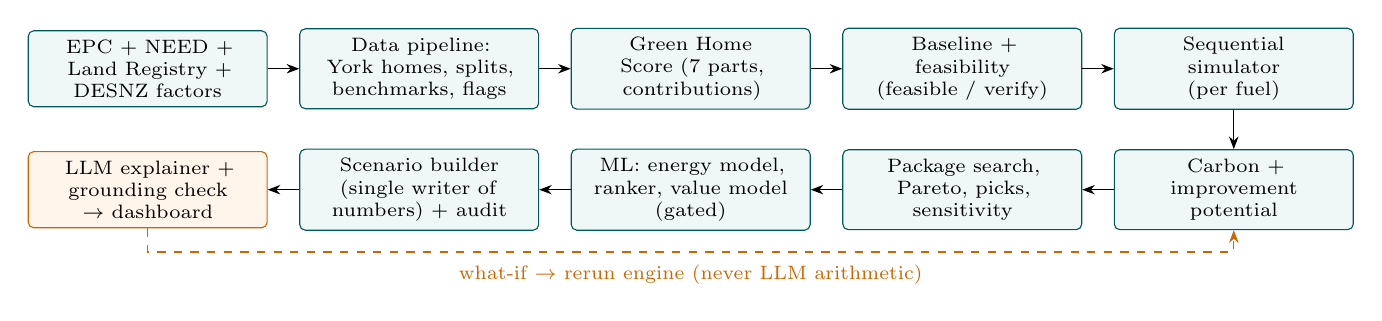
\begin{tikzpicture}[node distance=5mm and 4mm,
  box/.style={draw=teal!70!black,fill=teal!6,rounded corners=2pt,align=center,font=\scriptsize,minimum height=9mm,text width=28mm},
  llm/.style={box,draw=orange!80!black,fill=orange!8},
  >={Stealth[length=1.6mm]}]
\node[box] (data) {EPC + NEED +\\Land Registry +\\DESNZ factors};
\node[box,right=of data] (fe) {Data pipeline:\\York homes, splits,\\benchmarks, flags};
\node[box,right=of fe] (score) {Green Home\\Score (7 parts,\\contributions)};
\node[box,right=of score] (feas) {Baseline +\\feasibility\\(feasible / verify)};
\node[box,right=of feas] (sim) {Sequential\\simulator\\(per fuel)};
\node[box,below=of sim] (carb) {Carbon +\\improvement\\potential};
\node[box,left=of carb] (pkg) {Package search,\\Pareto, picks,\\sensitivity};
\node[box,left=of pkg] (ml) {ML: energy model,\\ranker, value model\\(gated)};
\node[box,left=of ml] (scen) {Scenario builder\\(single writer of\\numbers) + audit};
\node[llm,left=of scen] (llm) {LLM explainer +\\grounding check\\$\rightarrow$ dashboard};
\draw[->] (data)--(fe); \draw[->] (fe)--(score); \draw[->] (score)--(feas); \draw[->] (feas)--(sim);
\draw[->] (sim)--(carb); \draw[->] (carb)--(pkg); \draw[->] (pkg)--(ml); \draw[->] (ml)--(scen); \draw[->] (scen)--(llm);
\draw[->,dashed,orange!80!black] (llm.south) |- ++(0,-3mm) -| node[pos=0.25,below=1pt,font=\scriptsize]{what-if $\rightarrow$ rerun engine (never LLM arithmetic)} (carb.south);
\end{tikzpicture}
\end{center}
\vspace{-4pt}
\begin{itemize}
\item \textbf{Score:} documented, monotonic sub-score maps (e.g.\ SAP capped 0--100; intensity
$100\,(p_{90}-x)/(p_{90}-p_{10})$ with percentiles frozen on train only; element ratings 10/30/55/80/100). A missing part
is scored 50 with a [0,100] range and completeness $k/7$; $>2$ missing $\Rightarrow$ score unavailable.
\item \textbf{Feasibility:} catalogue rules (e.g.\ no loft for a flat with a dwelling above, no cavity fill after 2000,
no PV on flats); a missing input gives \emph{needs verification}, never \emph{infeasible}. ML may only reorder feasible measures.
\item \textbf{Simulator:} gas split into cooking (3.05\%, untouched) and space/water (77/23)\footnote{DESNZ, \emph{Energy Consumption in the UK 2026}, End-use data tables, Table U3 (domestic
natural gas by end use), mean of 2021--2025: cooking 3.05\%; space heating 77.3\% of space + water heating gas.}; NEED impacts
(\% of total gas) converted to the space-heating end use; fixed order fabric $\rightarrow$ glazing $\rightarrow$ controls
$\rightarrow$ heat pump (heat/SCOP 3.0 moves to electricity) $\rightarrow$ solar (grid import only). Reductions multiply.
\item \textbf{Carbon:} $\Delta C=\sum_{f\in\{elec,gas\}}\Delta E_f\cdot EF_f$ (0.14395 / 0.18231 kg CO$_2$e/kWh, DESNZ 2026).
\item \textbf{ML (in progress):} LightGBM energy model on NEED (replaces benchmarks only if it beats them), recommendation
ranker on EPC assessor recommendations, hedonic value model on 4,000 matched sales reported as an \emph{indicative} range (not causal),
enabled only after a manual match-precision gate ($\ge$0.90) and a held-out range-coverage check (75--85\%).
\item \textbf{LLM:} receives only the scenario JSON + audit and explains score, recommendations and trade-offs. It writes
placeholders only; code fills in every number from the scenario result.
\end{itemize}

\textbf{Status at M1:} data pipeline, score, feasibility, simulator, carbon, package search, sensitivity, audit and
scenario builder are implemented (169 passing tests, $\sim$1\,ms per home). Demo: an EPC-E 1970s house scores
\textbf{44/100 (Poor)}; its feasible package saves 20,957 kWh gas, adds 3,675 kWh electricity (heat pump), cuts
purchased energy by 68\% and carbon by 3.29\,t/yr; cheapest $\ge$10\% option: cavity-wall insulation (\pounds1,000).

\section{Planned testing methodology}
\begin{itemize}
\item \textbf{Leakage-safe splits:} property-level train/val/test (46,151 / 9,797 / 9,924); score percentiles and
models fitted on train only; no field unavailable at prediction time; EPC rating at sale taken only from earlier
certificates. Automated data checks (unique homes, split isolation, no zero-filled gaps, provenance).
\item \textbf{Hand-calculated reference suite:} energy balance with no retrofit; 3\% of 12,000\,kWh = 360\,kWh; loft+cavity
overlap $<$ sum; fabric-order invariance; full/partial/unknown heat pump (gas $\downarrow$, electricity $\uparrow$);
solar applied last; infeasible measure blocked; zero baseline $\Rightarrow$ unavailable; carbon signs. Demo homes are
reproduced from independent hand arithmetic to $10^{-6}$.
\item \textbf{Property tests:} monotonicity of every sub-score, class boundaries (29/30, 49/50, 64/65, 79/80), weights
sum to 1, per-fuel steps reconcile, same request $\Rightarrow$ same scenario ID.
\item \textbf{External validation:} simulated multi-measure packages vs NEED \emph{measured} combination savings
(tolerance $\pm$5\,pp). Our simulated combined savings \textbf{exceed} NEED's measured figures by 5.6--13.8 percentage
points, outside tolerance. We report this rather than tuning it away; likely causes include differences in home mix and
the gap between modelled and real behaviour. Single-measure NEED figures are model inputs, so they are not re-used as tests.
\item \textbf{Decision quality:} on held-out homes, compare three policies (fixed checklist, greedy, full package search)
under the same objective and budget (\pounds5k, \pounds15k, unlimited); report regret against the best package within
budget and feasibility violations. This measures performance under our documented simulator, not real-world optimality.
\item \textbf{ML:} validation metrics against simple baselines (benchmark medians for energy; rules-only ranking for
recommendations; precision@k, MAE); value range coverage on held-out sales.
\item \textbf{LLM:} held-out scenarios (missing/conflicting data, infeasible or interacting retrofits, electricity rising
after a heat pump, insufficient data). The LLM writes placeholders only; code fills in numbers from the scenario result.
A checker confirms no stray digits, that every placeholder exists, that the scenario ID matches, and that signs and
directions are correct; any failure falls back to a template. Targets: groundedness $\ge$90\%, factual accuracy $\ge$90\%, unsupported claims $<$5\%.
\item \textbf{Robustness:} one-at-a-time sensitivity (baseline $\pm$15\%, SCOP 2.5/3.5, gas split, impact low/high)
reporting whether recommendations survive; latency target $<$1\,s per scenario.
\end{itemize}
\end{document}
